\section{Organization and Management}
\label{sec:fdsp-tpcelec-management}

%%%%%%%%%%%%%%%%%%%%%%%%%%%%%%%%%%%
\subsection{Consortium Organization}
\label{sec:fdsp-tpcelec-management-consort}

At the moment the \dword{ce} consortium consists entirely of
US institutions, XX university groups plus groups from four
DOE national laboratories. A list of the participating institutions
and of the contact people in each institution is given in
Table~\ref{tab:SPCE:institutions}. The present consortium organization
structure includes a leader and a technical lead (both currently
from \fnal), with help on system design aspects from personnel
from BNL. A working group structure has been recently 
introduced with subgroups responsible for the detector 
components inside the cryostat (\dwords{asic}, \dwords{femb}, and
cold cables), outside the cryostat (mostly the \dwords{wiec} with 
their boards), plus a subgroup responsible for all the equipment
used for testing the detector components. When appropriate, subgroups
responsible for the integration activities at the \dword{itf} and
installation activities at \surf will also be formed (for the moment 
these activities are overseen by the technical lead). In addition
there will be a subgroup in charge of the software and physics
preparation activities, including calibrations and simulations.
Mechanical design activities span detector components both inside
and outside the cryostat and require strict contacts with both
technical coordination and other consortia (mainly the \dword{apa}
consortium). The lead engineer (from BNL) on mechanical aspects of the cold
electronics (mechanical interfaces with the \dwords{apa}, cabling, including 
cable trays, cryostat penetrations) works directly in contact with
the technical coordination team. The consortium will also have 
contact people for with the overall LBNF / DUNE management for
ES\&H and for QA/QC. For the moment these activities are mostly
overseen by the technical lead, with the expectation that they
will be transferred in part to the subgroup leader for the testing
activities. The list of current contact people for the various 
positions in the Consortium is listed in Table~\ref{tab:SPCE:leadership}.

\begin{dunetable}
[Participating intitutes]
{p{0.15\textwidth}p{0.75\textwidth}}
{tab:SPCE:institutions}
{Institutes participating in the Cold Electronics consortium}
ID & Institution (Contact person with E-mail) \\ \toprowrule
 1 & Brookhaven National Laboratory (\href{mailto:mworcester@bnl.gov}{Matt Worcester}) \\ \colhline
 2 & Boston University (\href{mailto:kearns@bu.edu}{Ed Kearns}) \\ \colhline
 3 & University of Chicago (\href{mailto:dwschmitz@uchicago.edu}{David Schmitz}) \\ \colhline
 4 & University of Cincinnati (\href{mailto:alex.sousa@uc.edu}{Alexander Sousa}) \\ \colhline
 5 & Colorado State University (\href{mailto:mrmooney@colostate.edu}{Michael Mooney}) \\ \colhline
 6 & Columbia University (\href{mailto:georgia@nevis.columbia.edu}{Georgia Karagiorgi}) \\ \colhline
 7 & University of California, Davis (\href{mailto:mulhearn@physics.ucdavis.edu}{Michael Mulhearn}) \\ \colhline
 8 & Fermi National Accelerator Laboratory (\href{mailto:dcc@fnal.gov}{David Christian}) \\ \colhline
 9 & University of Florida (\href{mailto:ikfuric@ufl.edu}{Ivan Furic}) \\ \colhline
10 & University of Hawaii (\href{mailto:varner@uhawaii.edu}{Gary Varner}) \\ \colhline
11 & Iowa State University (\href{mailto:krennrich@iastate.edu}{Frank Krennrich}) \\ \colhline
12 & University of California, Irvine (\href{mailto:bianjm@uci.edu}{Jianming Bian}) \\ \colhline
13 & Lawrence Berkeley National Laboratory (\href{mailto:cjslin@lbl.gov}{ChengJu Lin}) \\ \colhline
14 & Louisiana State University (\href{mailto:mtzanov@lsu.edu}{Martin Tzanov}) \\ \colhline
15 & Michigan State University (\href{mailto:bromberg@pa.msu.edu}{Carl Bromberg}) \\ \colhline
16 & University of Pennsylvania (\href{mailto:cmauger@penn.edu}{Christopher Mauger}) \\ \colhline
17 & SLAC National Accelerator Laboratory (\href{mailto:convery@slac.stanford.edu}{Mark Convery}) \\ \colhline
18 & Stony Brook University (\href{mailto:alpinist@nngroup.physics.sunysb.edu}{Chang Kee Jung}) \\
\end{dunetable}

\begin{dunetable}
[Leadership positions in the Consortium]
{p{0.45\textwidth}p{0.45\textwidth}}
{tab:SPCE:leadership}
{Current Leadership positions in the Cold Electronics consortium}\
Position & Responsible person (with E-mail) \\ \toprowrule
Leader & \href{mailto:dcc@fnal.gov}{David Christian} (Fermilab) \\ \colhline
Technical Lead & \href{mailto:mverzocc@fnal.gov}{Marco Verzocchi} (Fermilab) \\ \colhline
System Engineer & \href{mailto:chc@bnl.gov}{Hucheng Chen} (Brookhaven) \\ \colhline
Cold Components & \href{mailto:mverzocc@fnal.gov}{Marco Verzocchi} (Fermilab) \\ \colhline
Warm Components & \href{mailto:mworcester@bnl.gov}{Matt Worcester} (Brookhaven) \\ \colhline
Test Setups & \href{mailto:ikfuric@ufl.edu}{Ivan Furic} (Florida) \\ \colhline
Mechanical Design & \href{mailto:mzhao@bnl.gov}{Manhong Zhao} (Brookhaven) \\ \colhline
Reliability Task Force & \href{mailto:varner@uhawaii.edu}{Gary Varner} (Hawaii) \\ \colhline
TDR Editor & \href{mailto:mrmooney@colostate.edu}{Michael Mooney} (Colorado State) \\ \colhline
\end{dunetable}

In addition to the working groups task force on specific issues 
will be formed as necessary. A first example is the task force
charged with studying reliability issues in the \dword{ce} 
components and preparing recommendations for the choice of 
\dwords{asic}, the design of printed circuit boards, and testing. This 
working group will consider past experience from cryogenic detectors 
operated for a long time (ATLAS \lar calorimeters, NA48 liquid 
krypton calorimeter, HELIOS), from space-based experiments 
(FERMI/GLAST), and the lessons learned from \dword{pdsp} construction 
and commissioning. Input from other fields will also be sought. Later 
this working group will contribute to the development the \dword{qc} 
program for the \dword{ce} detector components, in collaboration
with the testing group leadership, starting from the \dword{pdsp} 
experience. At a later time a second task force, with a possible
personnel overlap with the first, and possibly including experts
from outside the DUNE Collaboration, will be formed to establish the
criteria for the \dword{asic} selection. This task force will
be charged with proposing a recommendation that will then go through
the DUNE Executive Board for the final approval.

%%%%%%%%%%%%%%%%%%%%%%%%%%%%%%%%%%%
\subsection{Planning Assumptions}
\label{sec:fdsp-tpcelec-management-planning}

Later in Section~\ref{sec:fdsp-tpcelec-management-cost} we describe
the current schedule for the construction, integration and installation
of the Cold Electronics detector components for the first Single
Phase TPC Far Detector. This schedule, and the cost associated
to the detector construction, are based on the experience gained
during the construction and commissioning of the \dword{pdsp}
detector. We have already discussed in Section~\ref{sec:fdsp-tpcelec-production-spares}
the number of spares parts that we are planning to fabricate to
account for known yield issues during the detector construction
and to address possible problems. Table~\ref{tab:SPCE:components}
gives a summary of all the components to be fabricated, and where
appropriate tested, that are required for the first Single Phase
TPC Far Detector.
To develop a schedule for the detector construction 
we have then considered the current state of the development of 
the \dwords{asic} and \dwords{femb} and of all the other components, 
and estimated the time required for the final developments of these
two components.

\begin{dunetable}[Number of Cold Electronics components required 
for the Single Phase TPC Far Detector]
{p{0.5\textwidth}p{0.5\textwidth}}
{tab:SPCE:components}
{Number of Cold Electronics components required for the Single 
Phase TPC Far Detector (accounting for spares and yield)}
Component & Number required \\ \toprowrule
FE ASIC & 30,000 chips (at least 77 wafers) \\ \colhline
ColdADC and COLDATA & 30,000 and 7,500 chips (at least 33 wafers) \\ \colhline
CRYO & 7,500 chips (at least 35 wafers) \\ \colhline
FEMB & 3,200 \\ \colhline
Cold signal cables & 1,650 and 1,575 (bottom and top \dword{apa}) \\ \colhline
Cold power cables & 1,650 and 1,575 (bottom and top \dword{apa}) \\ \colhline
Cold bias voltage cables & 660 and 630 (bottom and top \dword{apa}) \\ \colhline
Cryostat penetrations & 80 \\ \colhline
Cold Electronics flanges & 160 \\ \colhline
\dword{wiec} & 155 \\ \colhline
\dword{wib} & 775 \\ \colhline
\dword{ptc} & 155 \\ \colhline
Warm power cables & 165 (3 different lengths) \\ \colhline
Warm bias voltage cables & 1,320 (3 different lengths) \\ \colhline
Wiener PL506 power box & 30 \\ \colhline
Wiener MPOD crate & 30 \\ \colhline
Wiener MPOD modules with 8 HV channels & 180 \\ \colhline
Power supplies and cables for heaters and fans & 30 \\ \colhline
\end{dunetable}

We have also considered the possibility that a second detector may
be built using the Single Phase technology. In that case the construction
of the Cold Electronics components for the second detector would
immediately follow that of the first detector. The total number of
components for the second detector will be smaller than that of the
of the first detector under the assumption that for components inside
the cryostat the leftovers from the first detector can be used as
spares. Similarly for the components on the top of the cryostat the
pool of spares from the first detector should be sufficient to cover
also the second detector.

The critical path for the construction of the first Single Phase
TPC Far Detector is driven by the availability of the \dwords{femb},
which in turn depends on the completion of the design of the
\dwords{asic}. This is motivated by the fact that the construction
of the \dwords{apa} could start as early as in Spring, while the
decision on the \dword{asic}(s) to be used on the \dwords{femb}
may come as late as in Fall 2020. The schedule for this decision
is driven by the fact that the Cold Electronics consortium is
planning to complete a second design iteration on all the \dwords{asic}
and then to test various flavors of \dwords{femb} prior to taking
the decision. First version of all the \dwords{asic} will undergo
standalone tests in Spring 2019 and then will go through the 
sequence of system tests (with the 40\% \dword{apa} prototype at BNL,
with the seventh \dword{pd} \dword{apa} in the cold box at CERN,
and with the small TPC in the ICEBERG cryostat at Fermilab), which
will take place during Summer 2019, while at the same time lifetime
tests will be performed on all the \dwords{asic}. A review of the 
designs of the \dwords{asic} and \dwords{femb}, including results
from the system test stands and from lifetime tests will be done
in early Fall 2019, which will trigger eventual further design
changes on the \dwords{asic} and then the second round of prototyping
and testing. This leads to the Fall 2020 date for the final
\dword{asic} decision. This has the consequence that the initial
tests of the DUNE prototype \dwords{apa} will have to be performed
with preliminary versions of the \dwords{femb} that will still use
the first generation of \dwords{asic} while having the final 
mechanical and electrical connections to the \dwords{apa}.

After the review in Fall 2020 an additional six months may be 
required to have a final iteration on the \dword{femb} design
and a final round of system tests, before launching the fabrication
of the \dwords{asic} and of the \dwords{femb}. Engineering runs
for the \dwords{asic} and \dwords{femb} would take place in the
second half of 2021, with the bulk of the production starting in
the Spring of 2022. Depending on the chosen solution for the
\dwords{asic} the production and testing of all the chips required
for the construction of the first Single Phase TPC Far Detector
would be in hand by Spring or Summer 2023. The first batch of
production \dword{femb} would be available for installation on
the \dwords{apa} in Winter 2023, and the production would be
completed in Fall 2024, roughly six month after the completion
of the fabrication of the \dwords{apa} for the first detector.
This schedule assumes that during the construction of the 
\dwords{apa} integration tests will be performed using preliminary
versions of the \dwords{femb} that then will have to be replaced
with final ones at a later date. The integration of the \dwords{femb}
on the \dwords{apa} would be completed a couple of months after
the final set of \dwords{femb} is delivered at the \dword{itf}.

If a second Single Phase TPC Far Detector is built the critical
path at a certain point will transition from the \dwords{femb}
to the \dwords{apa}, under the assumption that both the construction
of the \dwords{apa} and of the \dwords{femb} will continue 
without interruption from that of the first detector. The reason
for this is that the construction of one \dword{apa} requires 
more time than that of the corresponding \dwords{femb}. Therefore
toward the end of the construction of a possible second detector
we expect that all the required \dwords{femb} will be at the
\dword{itf} waiting for the delivery of the \dwords{apa} before
the integration can take place.

All the other detector components that are a responsibility of the
Cold Electronics consortium can be produced on a relatively short
time-scale of less than two years. The procurement, assembly, and
testing of these components can be scheduled in such a way that
there is sufficient time in the schedule to address possible 
problems during the production phase. The changes of all these
components relative to those used in the \dword{pdsp} detector
are less important compared to those affecting the \dwords{asic}
and \dwords{femb} and the assumption is being made that final
designs for all the rest of the detector components will be 
available in the second half of 2020 and that production readiness
reviews will take place at the latest six months before the
\dword{asic} choice. The first components to be
required for installation of the detector are the cryostat 
penetrations, that need to be installed not later than the 
completion of the detector support structure inside the cryostat.
In this way the cryostat can be completely sealed except for
the manholes that are used to feed clear air inside the cryostat
and for the \dword{tco} that is used as exhaust for the air flow
and as entry point for the detector components. The rest of the
Cold Electronics components to be installed on top of the 
cryostat (\dwords{wiec} with all their boards, supplies, cables
and fibers) should be installed prior to the installation of
the corresponding rows of \dwords{apa}, in such a way that these
can be connected to power, control, and read-out and tested as
soon as they are installed. 

%%%%%%%%%%%%%%%%%%%%%%%%%%%%%%%%%%%
\subsection{Institutional Responsibilities}
\label{sec:fdsp-tpcelec-management-resp}

Design and prototyping activities for the \dword{sp} DUNE detector have 
been concentrated so far at the DOE national laboratories, mostly
because the focus was on the design of the new generation of 
\dwords{asic}. The design of the Front--End \dword{asic} was
done at Brookhaven, that of the CRYO chip at SLAC, while the
design of the new ColdADC was a joint effort of Brookhaven,
Fermilab and LBL. The COLDATA ASIC was designed at Fermilab, with
some components provided by engineers from the EE Department
at Southern Methodist University (not a consortium member).
In addition the design of the \dword{cts} was done at MSU.
For the construction of the \dword{pdsp} detector most of the
design and construction work was done at Brookhaven, with other
institutions contributing mostly to testing, installation and
commissioning. Given the extent of the project, mostly in
terms of testing additional institutions have started to contribute
to all the activities planned for the construction of then 
\dword{sp} detector starting in the middle of 2018. Most
of the engineering of detector components, with the exception
of the boards to be installed in the \dwords{wiec} and of
most boards and set-ups used for testing, will remain a responsibility
of the DOE national laboratories. Testing of components
(\dwords{asic}, \dwords{femb}, cables, power and bias voltage supplies,
\dwords{wiec} with their boards) will be performed at various
universities that are member of the Consortium. All institutions
are expected to contribute to the integration activities at
the \dword{itf} and to the installation at \surf, that is very
demanding in terms of personnel. A detailed list of the 
institutions contributing to the development, production, and
testing of the various detector components is given below.
\fixme{The assignment of responsibilities within the consortium
is still under discussion, with an expected first draft available
in January 2019. At that time additional information will be
added here.}

%%%%%%%%%%%%%%%%%%%%%%%%%%%%%%%%%%%
\subsection{High-Level Cost and Schedule}
\label{sec:fdsp-tpcelec-management-cost}

In Section~\ref{sec:fdsp-tpcelec-management-planning} we have 
discussed how the project will evolve from the current design
and prototyping phase to the production for the \dwords{asic}
and \dwords{femb} by the Spring of 2022. In the same time 
period the engineering of all other detector components will
be completed and prototypes fabricated, such that the procurement
and qualification of cold cables, cryostat penetrations, \dwords{wiec},
and power and bias voltage supplies, can start in Spring 2021.
Integration of the \dwords{femb} on the \dwords{apa} would then
take place on a period of 18 months starting in early 2023. At
this moment the installation and testing of the \dwords{apa} in 
the cryostat and the corresponding activities of the Cold
Electronics consortium, including the installation of all the
detector components on top of the cryostat, are scheduled to
take 10 months starting in Spring 20XX. A preliminary list of 
milestones indicating the current planning for the completion of 
the design, R\&D, and engineering phase, and then later for 
the production setup and the production, integration,
and installation activities is shown in Table~\ref{tab:SPCE:timeline}.

\begin{dunetable}
[\dword{ce} consortium milestones]
{p{0.15\textwidth}p{0.75\textwidth}}
{tab:SPCE:timeline}
{Milestones of the Cold Electronics consortium.}
\textbf{Date} & \textbf{Milestone} \\ \toprowrule
Feb 2019 & Complete the submission of the first generation of \dwords{asic} \\ \colhline
Aug 2019 & Complete the standalone testing of the first generation of \dwords{asic} \\ \colhline
Nov 2019 & Complete system and lifetime tests on the first generation of \dwords{asic} and \dwords{femb} \\ \colhline
Jan 2020 & Submission of second generation of \dwords{asic} \\ \colhline
Jul 2020 & Complete the standalone testing of the first generation of \dwords{asic} \\ \colhline
Nov 2020 & Complete system and lifetime tests on the second generation of \dwords{asic} and \dwords{femb} \\ \colhline
Nov 2020 & Decision on the \dword{asic}(s) to be used for construction \\ \colhline
May 2021 & Complete characterization of final prototypes of \dwords{asic} and \dwords{femb} including system tests \\  \colhline
Jul 2021 & Complete engineering design reviews and launch pre-production of detector components \\ \colhline 
Oct 2021 & Complete installation of \dwords{femb} on \dword{pdsp} \dwords{apa} \\ \colhline
Dec 2021 & Complete testing of pre-production of all \dwords{asic} \\ \colhline
Mar 2022 & Complete testing of pre-production \dwords{femb} \\ \colhline
Mar 2022 & Complete testing of prototypes and production readiness reviews \\ \colhline
May 2022 & Set-up of Cold Electronics test equipment at the \dword{itf} complete \\ \colhline
Feb 2023 & Begin installation of \dwords{femb} on \dwords{apa} at the \dword{itf} \\ \colhline
Mar 2023 & Procurement and testing of all detector components except \dwords{asic} and \dwords{femb} complete \\ \colhline
Aug 2023 & Construction and testing of \dwords{asic} complete \\ \colhline
Jan 2024 & Construction and testing of \dwords{femb} complete \\ \colhline
Sep 2024 & Integration of Cold Electronics components with \dwords{apa} complete \\ \colhline
Mar 20XX & Begin installation and testing of Cold Electronics components at \surf \\ \colhline
Jan 20YY & Installation of Cold Electronics components complete \\ \colhline
Aug 20YY & Complete testing and monitoring of detector prior to cryostat cool-down and filling \\ \colhline
Jun 20ZZ & Begin detector commissioning with cosmics \\ \colhline
Sep 20ZZ & Commissioning of detector complete \\ \colhline
\end{dunetable}

A detailed estimate of the Cold Electronics project costs has
been performed in Summer / Fall 2018 using as a starting point
the actual expenses for the construction of the \dword{pdsp}
detector. This puts the estimates of most costs on a very firm
basis, since most of the detector components will have only
minor changes relative to the \dword{pdsp} design. While the
set of \dwords{asic} used for the construction of the \dwords{femb}
is going to be completely, the cost of the \dwords{femb} can
be estimated reliably using the \dword{pdsp} estimation,
once the cost of the FPGA is subtracted from the total,
since the fabrication cost of the printed circuit board,
the cost of the discrete components, and the assembly cost
are not going to be significantly different. The same holds
for the \dwords{wib} that may be altered significantly.
The cost drivers in the case of the \dwords{wib} are the
printed circuit board fabrication, the components (including
optical transmitters and receivers that are not going to change),
the FPGA, and the assembly. The \dwords{asic}' set is going to
be completely new, but the fabrication costs are actually
known rather well, as the prototyping and fabrication of
\dwords{asic} are performed through frame contracts, either
through MOSIS in the USA or through IMEC in Europe, which
have a fixed costs for production and costs in the engineering
phase that depend only on the size of the chip. One item that
undergoes a significant change for DUNE is the cryostat penetration,
where the spool piece changes from a T--shape to a cross--shape.
Even before completing the engineering of the spool piece
the cost increase can be estimated rather reliably, just by
scaling the cost by a 33% factor that reflects the increase
in the amount of tubing and of welding necessary to build
the spool piece. 

Overall the biggest uncertainty in the cost of the project is
in the prototyping phase, where we assume that only a second
iteration of \dwords{asic}' and \dwords{femb} prototypes
is necessary prior to moving to the pre-production of 
components. The other main uncertainty in the cost of the
project is related to the preparation of all the testing
equipment required both during the prototyping phase and
during the construction and qualification of the detector
components. These cost uncertainties are not sizable 
relative to the overall cost of all the Cold Electronics
detector components.

An estimate of the construction costs for the first Single Phase
TPC Far Detector, including all the costs in the prototyping and
pre-production phases starting from January 2020 is given in Table~\ref{tab:SPCE:costs}.
\fixme{This is for the moment a place holder. There has to
be an agreement with the Neutrino Cost Group on how to present
these costs, and whether only CORE costs should be presented in
this table. The table format below is a proposal from the
Cold Electronics consortium that needs to be discussed with
the DUNE management and with the NCG. The starting date also
needs to be discussed.}

\begin{dunetable}
[Construction costs for the Cold Electronics detector components]
{lrrr}
{tab:SPCE:costs}
{Construction costs for the Cold Electronics detector components during the various phases of the project}
Component & Prototyping & Pre--production & Production \\ \toprowrule
\dwords{asic} & & & \\ \colhline
\dwords{femb} & & & \\ \colhline
Cold cables & & & \\ \colhline
Cryostat penetrations & & & \\ \colhline
\dwords{wiec}, \dwords{wib}, \dwords{ptc} & & & \\ \colhline
Power and bias voltage supplies & & & \\ \colhline
Test stands & & & \\ \colhline
Integration & & & \\ \colhline
Installation & & & \\ \colhline
\end{dunetable} 

The estimates for the labor needs are also based on the
experience from the \dword{pdsp} construction. The assumption
is made that the capability of testing multiple \dwords{asic}
at once and the automatization of the testing process itself,
both for \dwords{asic} and \dwords{femb}, will result in
a reduction of the personnel need for these tasks. The
integration activities at the \dword{itf} and at \surf
will be more complex than those for \dword{pdsp} and
will require more personnel. A complete estimate of the
personnel needs for the integration and installation tasks
requires a better definition of the responsibilities of
the various consortia (\dword{apa}, \dword{hv}, \dword{pds},
\dword{daq}, and \dword{cisc}) and of the underground
installation team for all the activities that take place
at \surf. The personnel needs for the project are listed in
Table~\ref{tab:SPCE:personnel} for the prototyping,
pre-production and construction phases. The personnel
needs are expressed in terms of full-time equivalent
people (FTE) for each of five job categories: graduate students,
post-docs, scientists, engineers, technicians. The
integral number of FTE--years in each job category is given
in the table. Distributions of the number of FTEs as
a function of time, without differentiation between the
phases of the project are given in Figure~\ref{fig:SPCE:ftedist}.
\fixme{The format of the table needs to be agreed upon with
the DUNE management and the Neutrino Cost Group. This table
will not be available before Spring 2019, as it depends on
the update of the DOE project schedule, that will happen on
that scale. The figure mentioned in the text will be made
available at the same time. The current one is a temporary 
place holder.}

\begin{dunefigure}
[Personnel needs for the Cold Electronics construction as a function of time]
{fig:SPCE:ftedist}
{Personnel needs for the construction of the Cold Electronics detector components 
as a function of time for different job categories.}
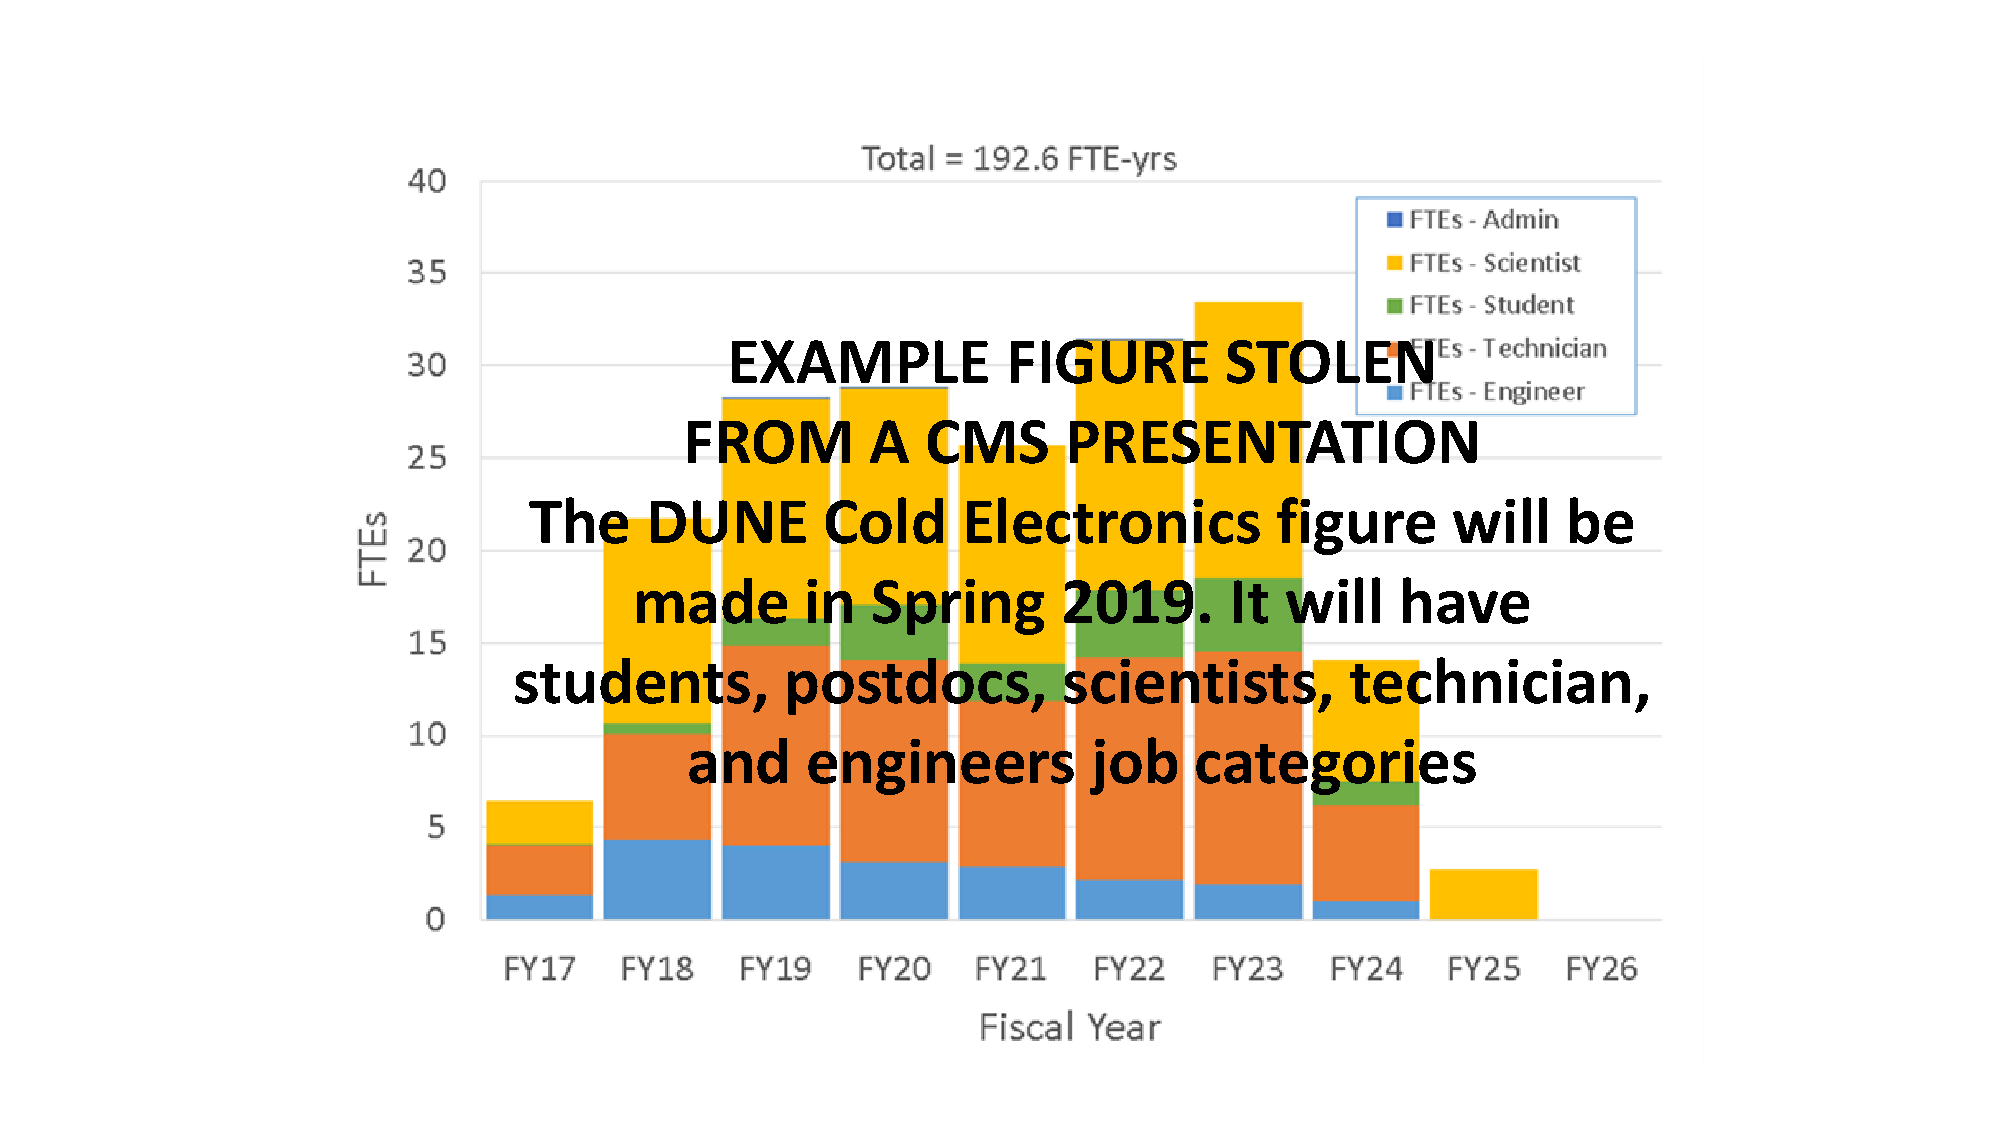
\includegraphics[width=0.8\linewidth]{sp-tpcelec-personnel-vs-time.pdf}
\end{dunefigure}

\begin{dunetable}
[Personnel needs for the Cold Electronics consortium]
{lrrrrr}
{tab:SPCE:costs}
{Personnel needs (in FTE--years) for the construction of the Cold Electronics detector 
components, their integration and installation for different job categories and 
in different project phases}
Component & Students & Postdocs & Scientists & Engineers & Technicians \\
\rowcolor{dunetablecolor}
\multicolumn{6}{c}{Prototyping phase} \\ \toprowrule
\dwords{asic} & & & & & \\ \colhline
\dwords{femb} & & & & &  \\ \colhline
Cold cables & & & & & \\ \colhline
Cryostat penetrations & & & & & \\ \colhline
\dwords{wiec}, \dwords{wib}, \dwords{ptc} & & & & & \\ \colhline
Power and bias voltage supplies & & & & & \\ \colhline
Test stands & & & & & \\ 
\rowcolor{dunetablecolor}
\multicolumn{6}{c}{Pre--production phase} \\ \toprowrule
\dwords{asic} & & & & & \\ \colhline
\dwords{femb} & & & & &  \\ \colhline
Cold cables & & & & & \\ \colhline
Cryostat penetrations & & & & & \\ \colhline
\dwords{wiec}, \dwords{wib}, \dwords{ptc} & & & & & \\ \colhline
Power and bias voltage supplies & & & & & \\ \colhline
Test stands & & & & & \\ \colhline
Integration & & & & & \\
\rowcolor{dunetablecolor}
\multicolumn{6}{c}{Construction phase} \\ \toprowrule
\dwords{asic} & & & & & \\ \colhline
\dwords{femb} & & & & &  \\ \colhline
Cold cables & & & & & \\ \colhline
Cryostat penetrations & & & & & \\ \colhline
\dwords{wiec}, \dwords{wib}, \dwords{ptc} & & & & & \\ \colhline
Power and bias voltage supplies & & & & & \\ \colhline
Test stands & & & & & \\ \colhline
Integration & & & & & \\ \colhline
Installation & & & & & \\ \colhline
\end{dunetable}
